\section{Configuración inicial} \label{configuracion}
\subsection{Componentes} \label{componentes}
El dispositivo CABRA cuenta con una parte de hardware y una parte de software.
Su hardware está compuesto por:
\begin{itemize}
    \item Placa de adquisición de datos.
    \item Auriculares de conducción aérea.
    \item Auriculares de conducción ósea.
    \item Electrodos de superficie.
    \item Cable de conexión USB.
    \item Cable de conexión de electrodos.
    \item Carcasa de protección.
\end{itemize}

El software de CABRA es un programa de computadora que se debe instalar en una computadora con sistema operativo Windows 7 o superior.
Se debe contar además con un puerto USB disponible para conectar la placa de adquisición de datos.

\subsection{Instalación del software} \label{instalacion}

Para instalar el software de CABRA, se debe seguir los siguientes pasos:
\begin{enumerate}
    \item Descargar el instalador del software de CABRA desde el siguiente enlace: \url{https://www.cabra.com.ar}.
    \item Ejecutar el instalador y seguir las instrucciones que aparecen en pantalla.
    \item Conectar la placa de adquisición de datos a un puerto USB de la computadora.
    \item Abrir el software de CABRA.
\end{enumerate}

\subsection{Configuración de la placa de adquisición de datos} \label{configuracion_placa}

El primer paso para la configuración de la placa de adquisición es la correcta colocación de los electrodos.
Como se muestra en la Figura \ref{fig:electrodos}, los electrodos deben colocarse en la cabeza del paciente de la siguiente manera:
\begin{itemize}
    \item Electrodo de activo ($V_{in}^{+}$): en la frente del paciente.
    \item Electrodo de tierra ($V_{in}^{-}$): en la apófisis mastoides ipsilateral del paciente.
    \item Electrodo de referencia (neutro): en la apófisis mastoides contralateral del paciente.
\end{itemize}

\begin{figure}[H]
    \centering
    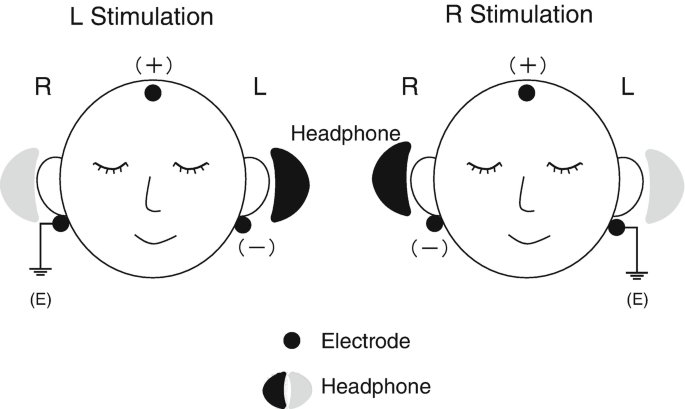
\includegraphics[width=0.5\textwidth]{figuras/electrodos.png}
    \caption{Colocación de los electrodos en la cabeza del paciente, para mediciones de ABR en oido izquierdo (L) o derecho (R).}
    \label{fig:electrodos}
\end{figure}

Luego, encastrar el pin metálico de los electrodos a la ficha hembra de los cables de adquisición.
Finalmente, conectar los cables de adquisición a la placa de adquisición de datos, mediante la entrada auxiliar.
\textit{Observación}: Para evaluar un oído luego de haber evaluado el contraleteral, no desconectar los electrodos
ya colocados.
Simplemente, desencastar los electrodos de la ficha hembra de los cables de adquisición y conectar los electrodos del otro oído.

\subsection{Configuración de los auriculares} \label{configuracion_auriculares}

Los auricuales, sean de conducción ósea o aérea, deben ir conectados a la computadora.
Es vital que se setee el volumen al máximo para realizar las pruebas.
Evitar confusiones de lado para los auriculares, verificando que el canal izquierdo se conecte al oido izquierdo y
viceversa.